% =====================================================================
% 波浪能最大输出功率设计 —— 图表 LaTeX 引用片段
% 用法：\usepackage{float} \usepackage{booktabs} \usepackage{graphicx}
% 在正文中 % =====================================================================
% 波浪能最大输出功率设计 —— 图表 LaTeX 引用片段
% 用法：\usepackage{float} \usepackage{booktabs} \usepackage{graphicx}
% 在正文中 % =====================================================================
% 波浪能最大输出功率设计 —— 图表 LaTeX 引用片段
% 用法：\usepackage{float} \usepackage{booktabs} \usepackage{graphicx}
% 在正文中 % =====================================================================
% 波浪能最大输出功率设计 —— 图表 LaTeX 引用片段
% 用法：\usepackage{float} \usepackage{booktabs} \usepackage{graphicx}
% 在正文中 \input{figures/latex_includes.tex}
% =====================================================================

% ---- 图 1：浮子与振子垂荡位移时程 ----
\begin{figure}[H]
    \centering
    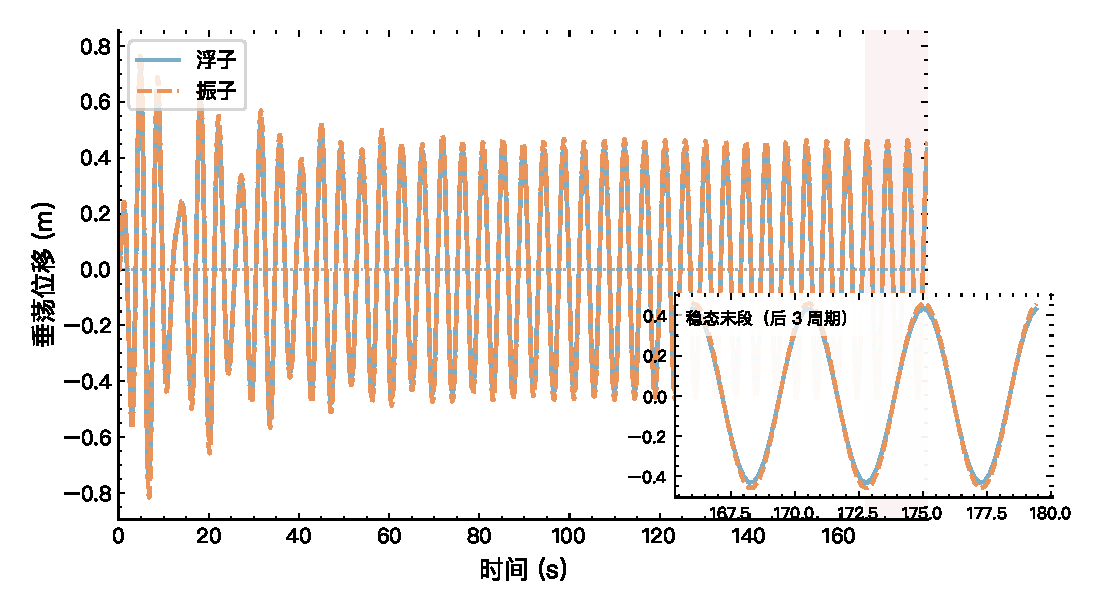
\includegraphics[width=0.85\textwidth]{figures/fig_1_heave_displacement.pdf}
    \caption{浮子与振子垂荡位移时程（前 40 个波浪周期，线性阻尼）}
    \label{fig:heave_displacement}
\end{figure}

% ---- 图 2：浮子与振子垂荡速度时程 ----
\begin{figure}[H]
    \centering
    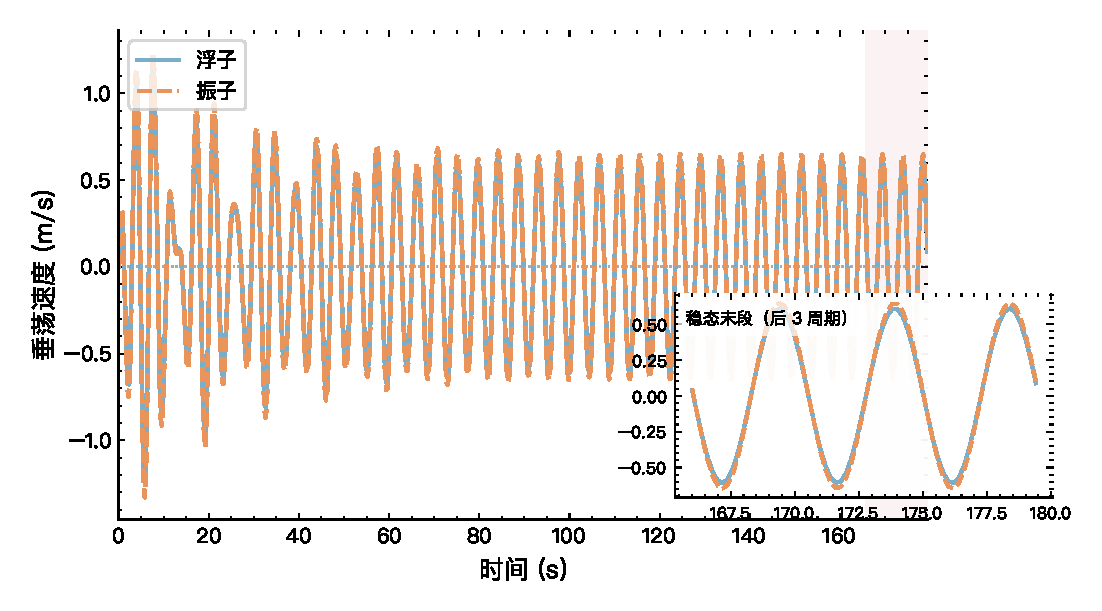
\includegraphics[width=0.85\textwidth]{figures/fig_2_heave_velocity.pdf}
    \caption{浮子与振子垂荡速度时程（前 40 个波浪周期，线性阻尼）}
    \label{fig:heave_velocity}
\end{figure}

% ---- 图 3：相对位移与相对速度时程 ----
\begin{figure}[H]
    \centering
    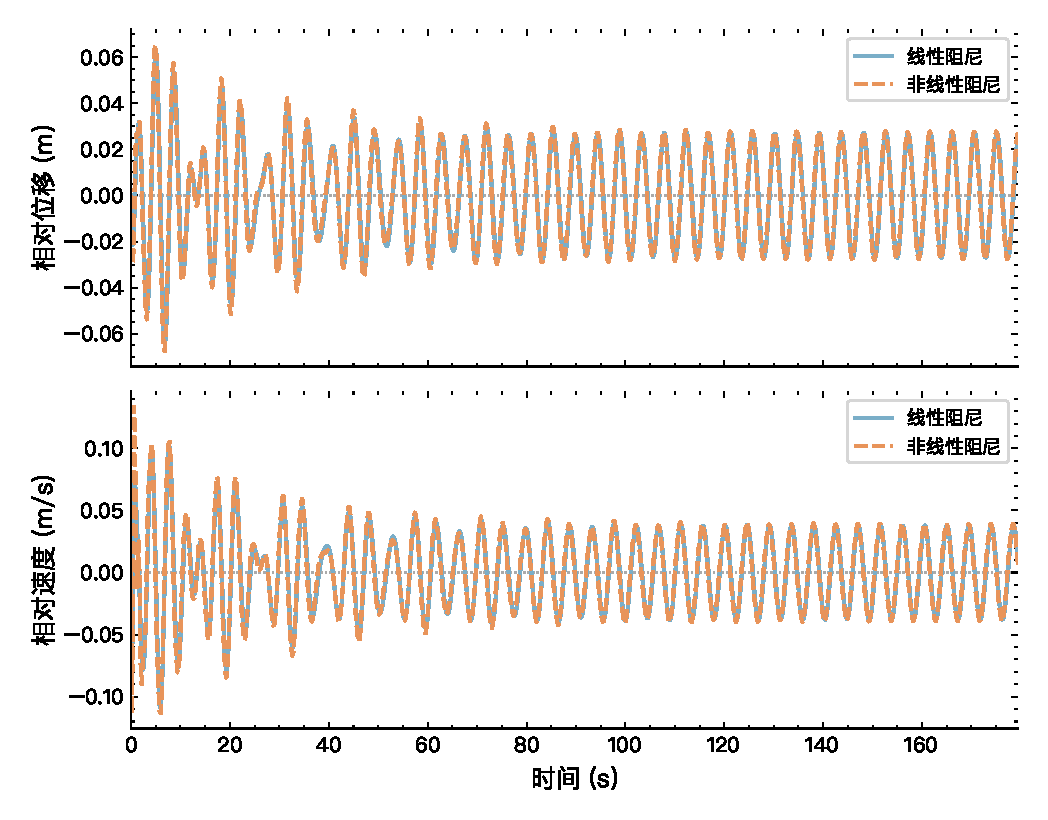
\includegraphics[width=0.85\textwidth]{figures/fig_3_relative_motion.pdf}
    \caption{浮子与振子相对位移及相对速度时程（线性与非线性阻尼对比）}
    \label{fig:relative_motion}
\end{figure}

% ---- 图 4：PTO 瞬时功率曲线 ----
\begin{figure}[H]
    \centering
    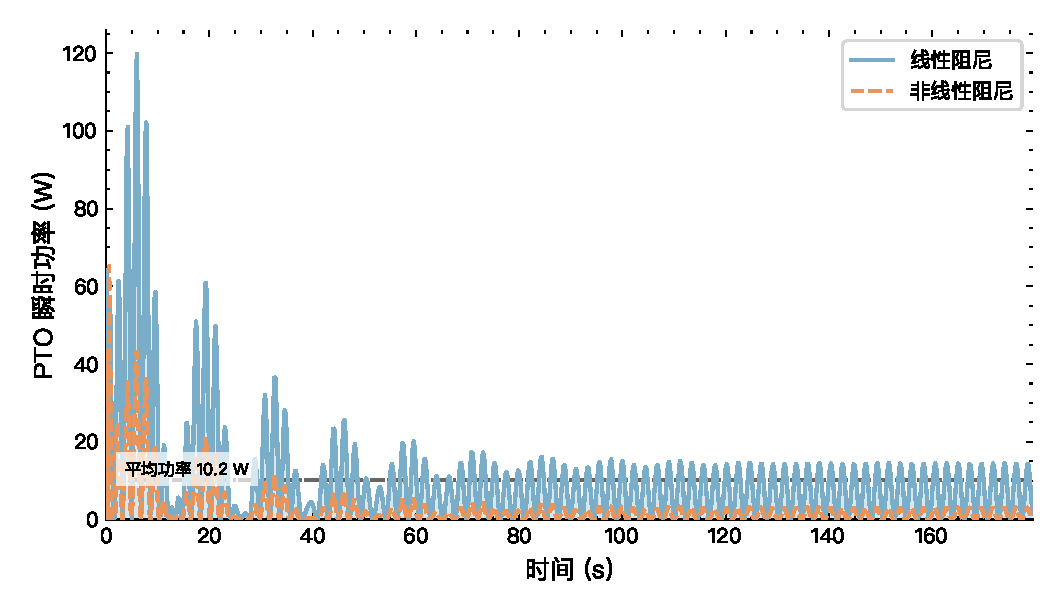
\includegraphics[width=0.85\textwidth]{figures/fig_4_pto_power.pdf}
    \caption{PTO 瞬时输出功率曲线（线性与非线性阻尼对比）}
    \label{fig:pto_power}
\end{figure}

% ---- 表 1：优化结果汇总 ----
\input{figures/TABLE_summary.tex}

% ---- 表 2：问题1 指定时刻快照 ----
\input{figures/TABLE_snapshot.tex}

% =====================================================================

% ---- 图 1：浮子与振子垂荡位移时程 ----
\begin{figure}[H]
    \centering
    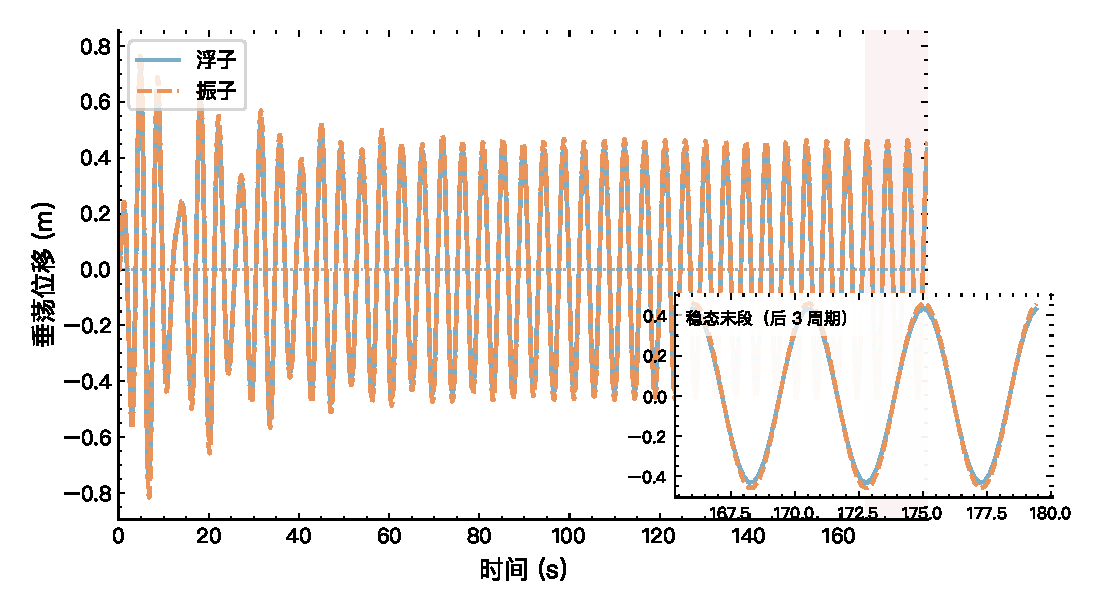
\includegraphics[width=0.85\textwidth]{figures/fig_1_heave_displacement.pdf}
    \caption{浮子与振子垂荡位移时程（前 40 个波浪周期，线性阻尼）}
    \label{fig:heave_displacement}
\end{figure}

% ---- 图 2：浮子与振子垂荡速度时程 ----
\begin{figure}[H]
    \centering
    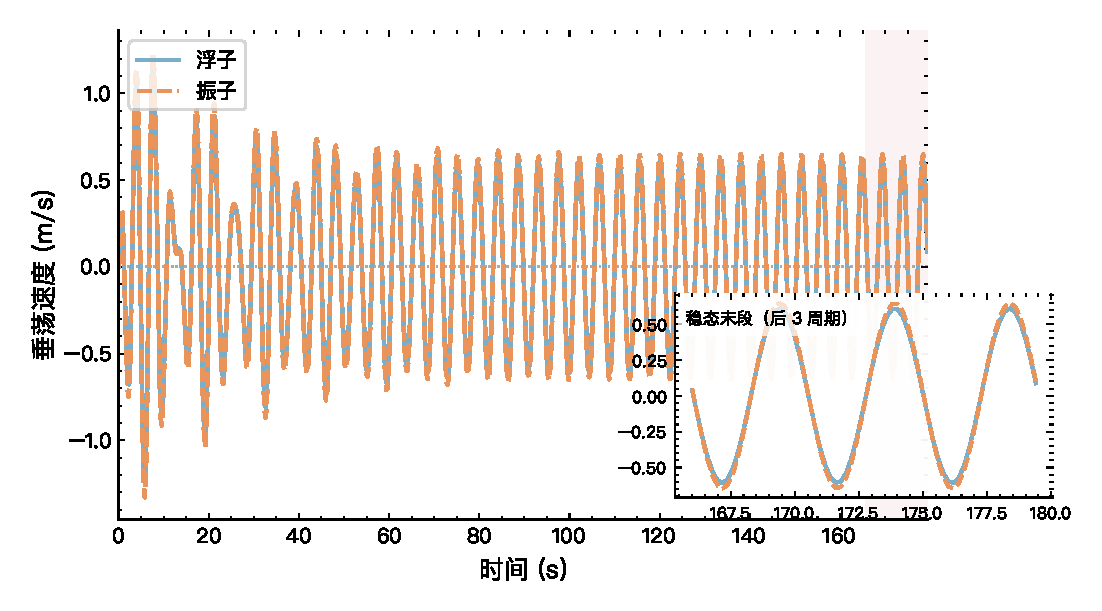
\includegraphics[width=0.85\textwidth]{figures/fig_2_heave_velocity.pdf}
    \caption{浮子与振子垂荡速度时程（前 40 个波浪周期，线性阻尼）}
    \label{fig:heave_velocity}
\end{figure}

% ---- 图 3：相对位移与相对速度时程 ----
\begin{figure}[H]
    \centering
    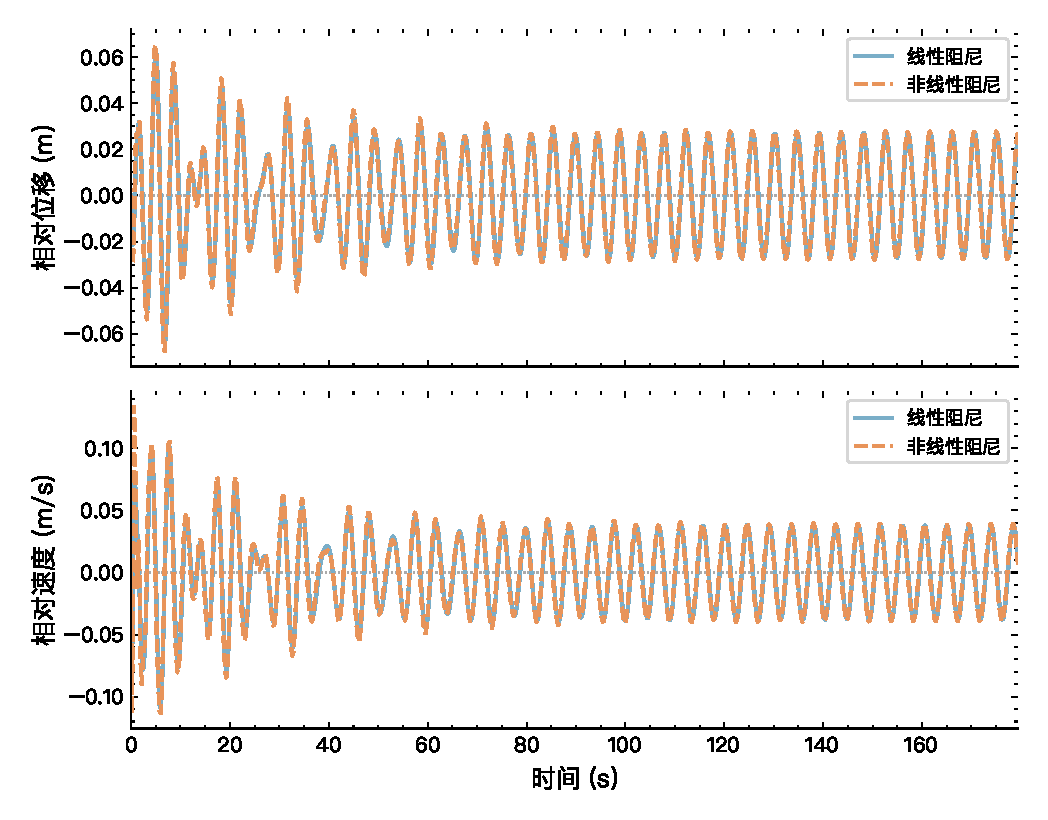
\includegraphics[width=0.85\textwidth]{figures/fig_3_relative_motion.pdf}
    \caption{浮子与振子相对位移及相对速度时程（线性与非线性阻尼对比）}
    \label{fig:relative_motion}
\end{figure}

% ---- 图 4：PTO 瞬时功率曲线 ----
\begin{figure}[H]
    \centering
    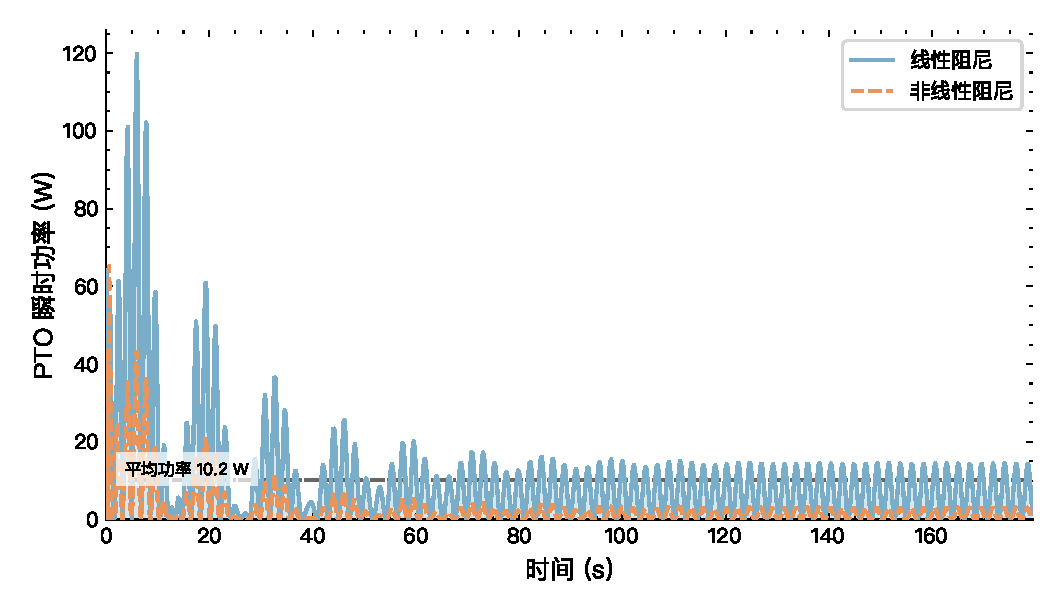
\includegraphics[width=0.85\textwidth]{figures/fig_4_pto_power.pdf}
    \caption{PTO 瞬时输出功率曲线（线性与非线性阻尼对比）}
    \label{fig:pto_power}
\end{figure}

% ---- 表 1：优化结果汇总 ----
% 各子问题能量输出优化结果汇总
\begin{table}[H]
\centering
\caption{各子问题能量输出优化结果汇总}
\label{tab:opt_summary}
\begin{tabular}{lcc}
\toprule
子问题 & 最优阻尼 & 最大平均输出功率 (W) \\
\midrule
问题2（线性） & $C^*=3.72\times10^4$ N·s/m & 229.334 \\
问题2（非线性） & $\alpha^*=1.0\times10^5$, $P^*=0.417$ & 229.980 \\
问题4（直线） & $C_z^*=5.92\times10^4$ N·s/m & 318.336 \\
问题4（旋转） & $C_\theta^*=1.0\times10^5$ N·m·s & 0.011 \\
\midrule
问题4 合计 & — & 318.347 \\
\bottomrule
\end{tabular}
\end{table}


% ---- 表 2：问题1 指定时刻快照 ----
% 问题1 指定时刻浮子/振子位移与速度快照（线性阻尼）
\begin{table}[H]
\centering
\caption{问题1 指定时刻浮子与振子位移/速度快照（线性阻尼 $C=10^4$ N·s/m）}
\label{tab:snapshot}
\resizebox{\textwidth}{!}{%
\begin{tabular}{lcccc}
\toprule
时间 $t$ (s) & 浮子位移 (m) & 浮子速度 (m/s) & 振子位移 (m) & 振子速度 (m/s) \\
\midrule
10  & $-0.1907$ & $-0.6410$ & $-0.2117$ & $-0.6940$ \\
20  & $-0.5907$ & $-0.2410$ & $-0.6342$ & $-0.2728$ \\
40  & $0.2854$  & $0.3130$  & $0.2965$  & $0.3329$  \\
60  & $-0.3145$ & $-0.4795$ & $-0.3314$ & $-0.5157$ \\
100 & $-0.0836$ & $-0.6042$ & $-0.0841$ & $-0.6430$ \\
\bottomrule
\end{tabular}}
\end{table}


% =====================================================================

% ---- 图 1：浮子与振子垂荡位移时程 ----
\begin{figure}[H]
    \centering
    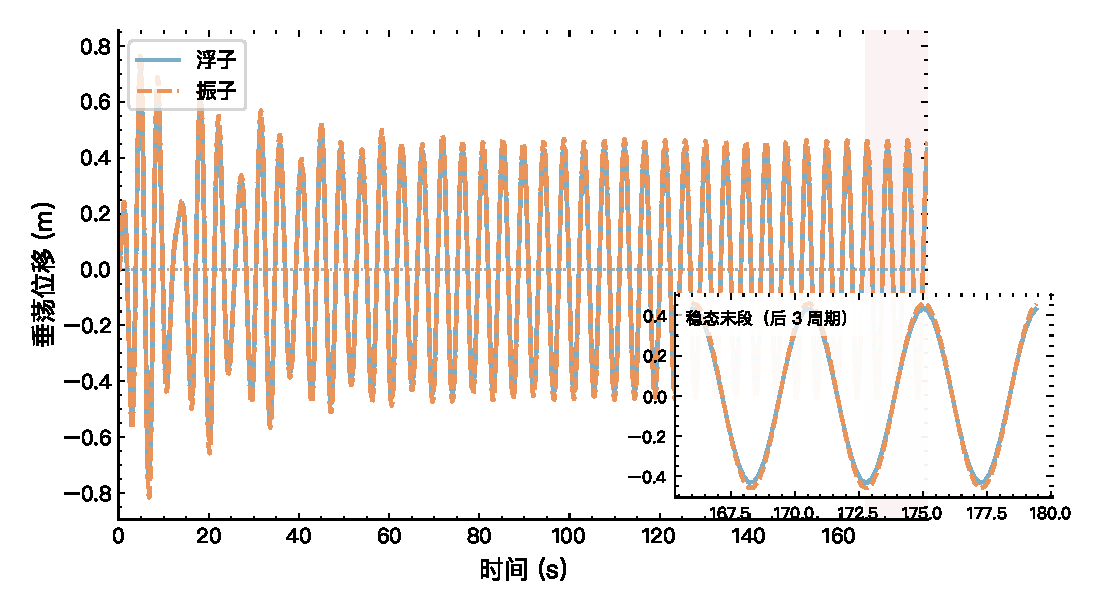
\includegraphics[width=0.85\textwidth]{figures/fig_1_heave_displacement.pdf}
    \caption{浮子与振子垂荡位移时程（前 40 个波浪周期，线性阻尼）}
    \label{fig:heave_displacement}
\end{figure}

% ---- 图 2：浮子与振子垂荡速度时程 ----
\begin{figure}[H]
    \centering
    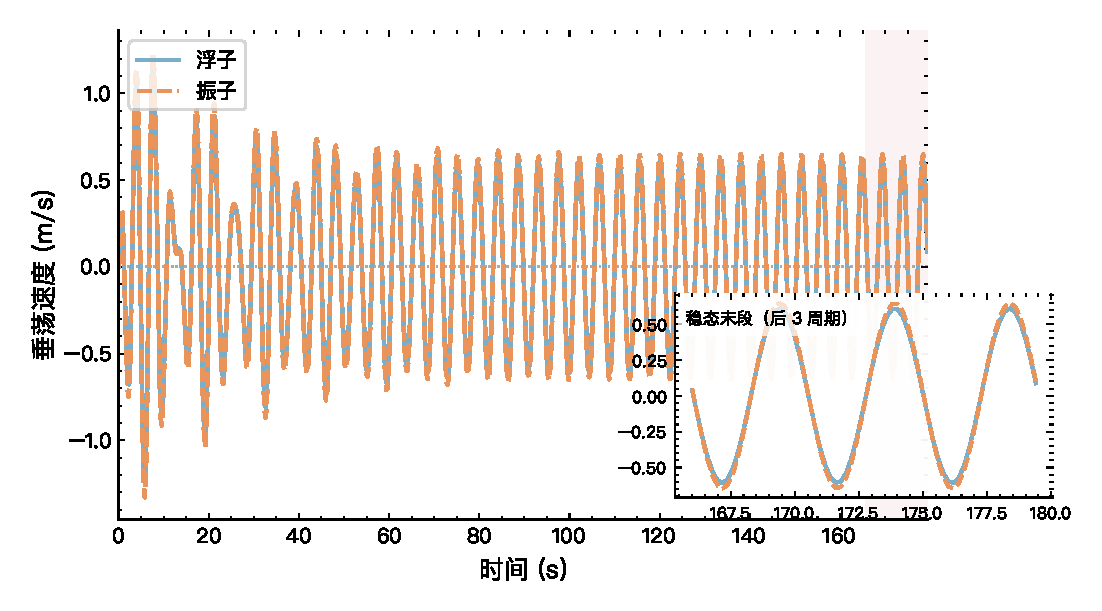
\includegraphics[width=0.85\textwidth]{figures/fig_2_heave_velocity.pdf}
    \caption{浮子与振子垂荡速度时程（前 40 个波浪周期，线性阻尼）}
    \label{fig:heave_velocity}
\end{figure}

% ---- 图 3：相对位移与相对速度时程 ----
\begin{figure}[H]
    \centering
    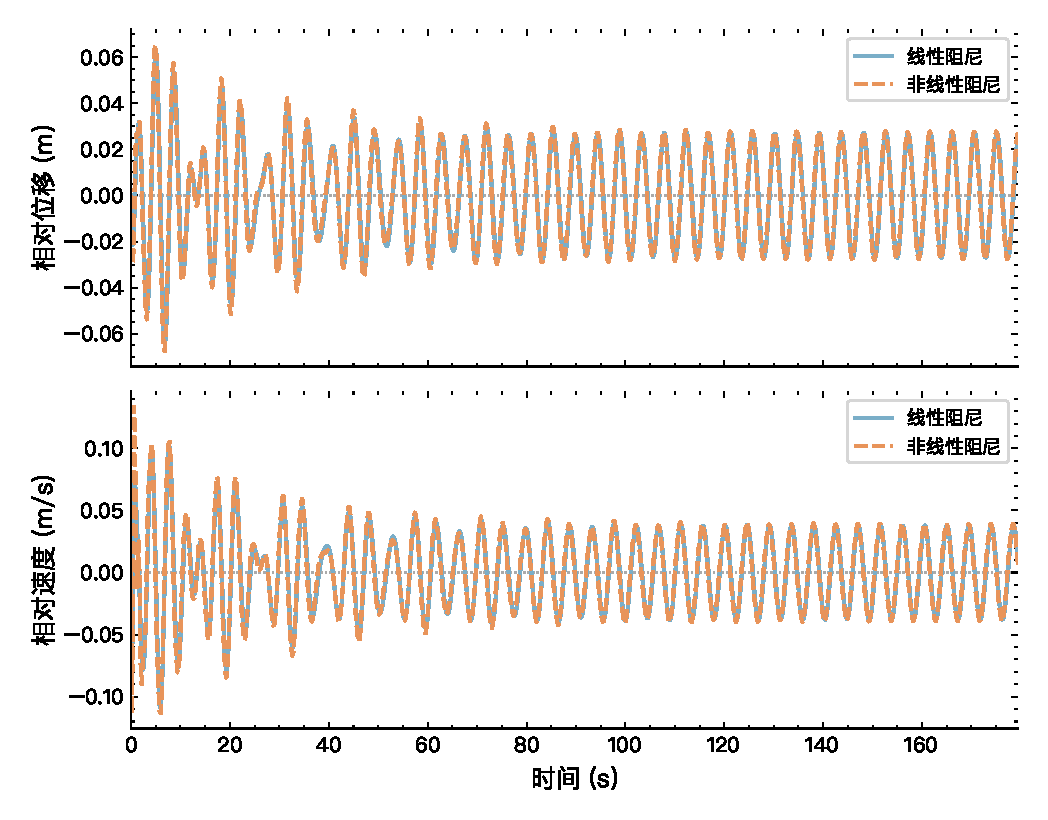
\includegraphics[width=0.85\textwidth]{figures/fig_3_relative_motion.pdf}
    \caption{浮子与振子相对位移及相对速度时程（线性与非线性阻尼对比）}
    \label{fig:relative_motion}
\end{figure}

% ---- 图 4：PTO 瞬时功率曲线 ----
\begin{figure}[H]
    \centering
    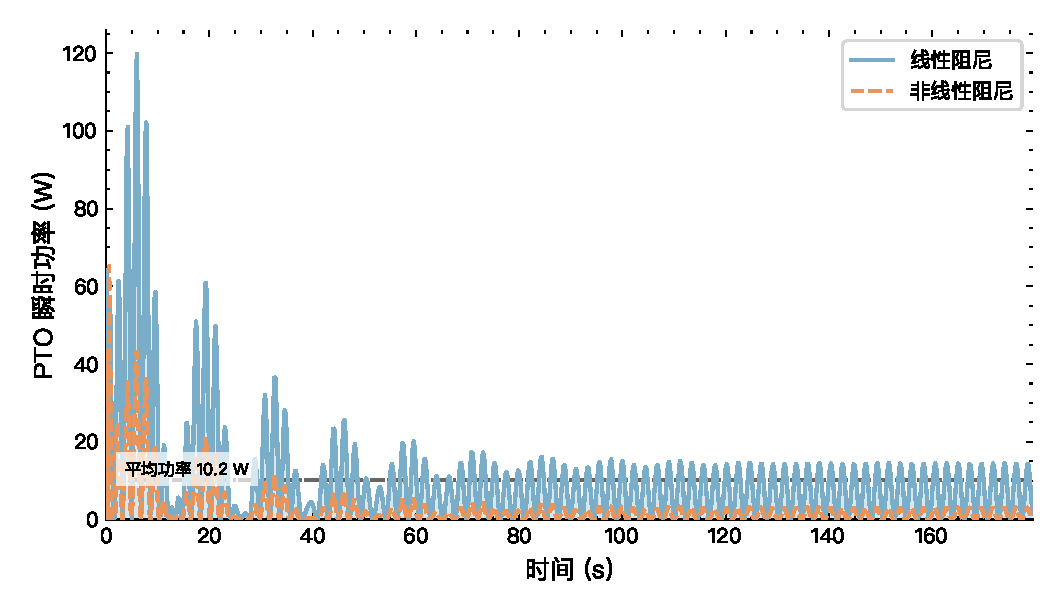
\includegraphics[width=0.85\textwidth]{figures/fig_4_pto_power.pdf}
    \caption{PTO 瞬时输出功率曲线（线性与非线性阻尼对比）}
    \label{fig:pto_power}
\end{figure}

% ---- 表 1：优化结果汇总 ----
% 各子问题能量输出优化结果汇总
\begin{table}[H]
\centering
\caption{各子问题能量输出优化结果汇总}
\label{tab:opt_summary}
\begin{tabular}{lcc}
\toprule
子问题 & 最优阻尼 & 最大平均输出功率 (W) \\
\midrule
问题2（线性） & $C^*=3.72\times10^4$ N·s/m & 229.334 \\
问题2（非线性） & $\alpha^*=1.0\times10^5$, $P^*=0.417$ & 229.980 \\
问题4（直线） & $C_z^*=5.92\times10^4$ N·s/m & 318.336 \\
问题4（旋转） & $C_\theta^*=1.0\times10^5$ N·m·s & 0.011 \\
\midrule
问题4 合计 & — & 318.347 \\
\bottomrule
\end{tabular}
\end{table}


% ---- 表 2：问题1 指定时刻快照 ----
% 问题1 指定时刻浮子/振子位移与速度快照（线性阻尼）
\begin{table}[H]
\centering
\caption{问题1 指定时刻浮子与振子位移/速度快照（线性阻尼 $C=10^4$ N·s/m）}
\label{tab:snapshot}
\resizebox{\textwidth}{!}{%
\begin{tabular}{lcccc}
\toprule
时间 $t$ (s) & 浮子位移 (m) & 浮子速度 (m/s) & 振子位移 (m) & 振子速度 (m/s) \\
\midrule
10  & $-0.1907$ & $-0.6410$ & $-0.2117$ & $-0.6940$ \\
20  & $-0.5907$ & $-0.2410$ & $-0.6342$ & $-0.2728$ \\
40  & $0.2854$  & $0.3130$  & $0.2965$  & $0.3329$  \\
60  & $-0.3145$ & $-0.4795$ & $-0.3314$ & $-0.5157$ \\
100 & $-0.0836$ & $-0.6042$ & $-0.0841$ & $-0.6430$ \\
\bottomrule
\end{tabular}}
\end{table}


% =====================================================================

% ---- 图 1：浮子与振子垂荡位移时程 ----
\begin{figure}[H]
    \centering
    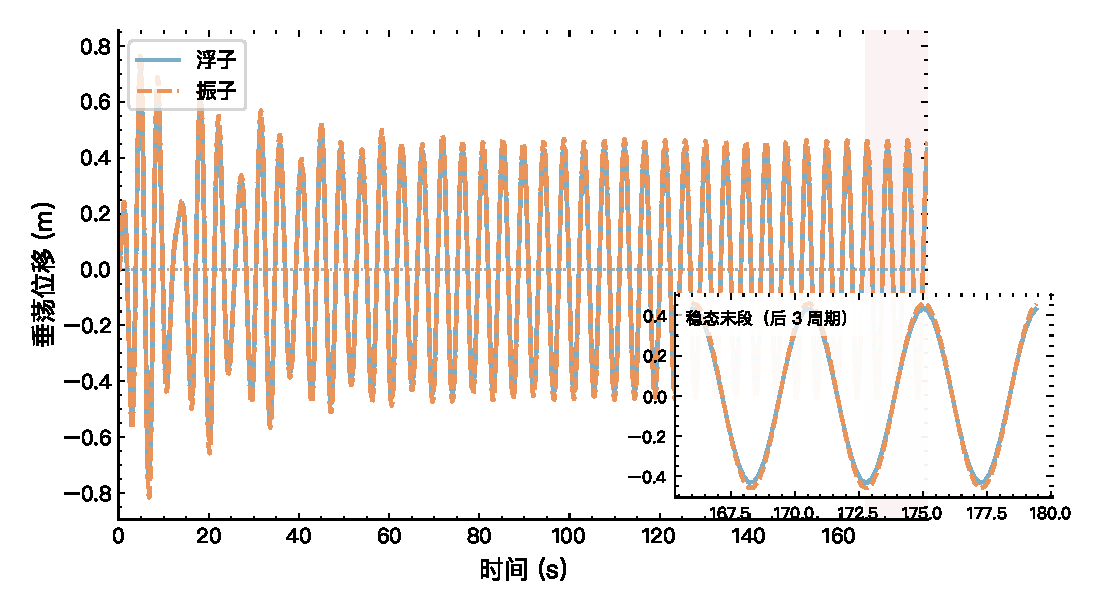
\includegraphics[width=0.85\textwidth]{figures/fig_1_heave_displacement.pdf}
    \caption{浮子与振子垂荡位移时程（前 40 个波浪周期，线性阻尼）}
    \label{fig:heave_displacement}
\end{figure}

% ---- 图 2：浮子与振子垂荡速度时程 ----
\begin{figure}[H]
    \centering
    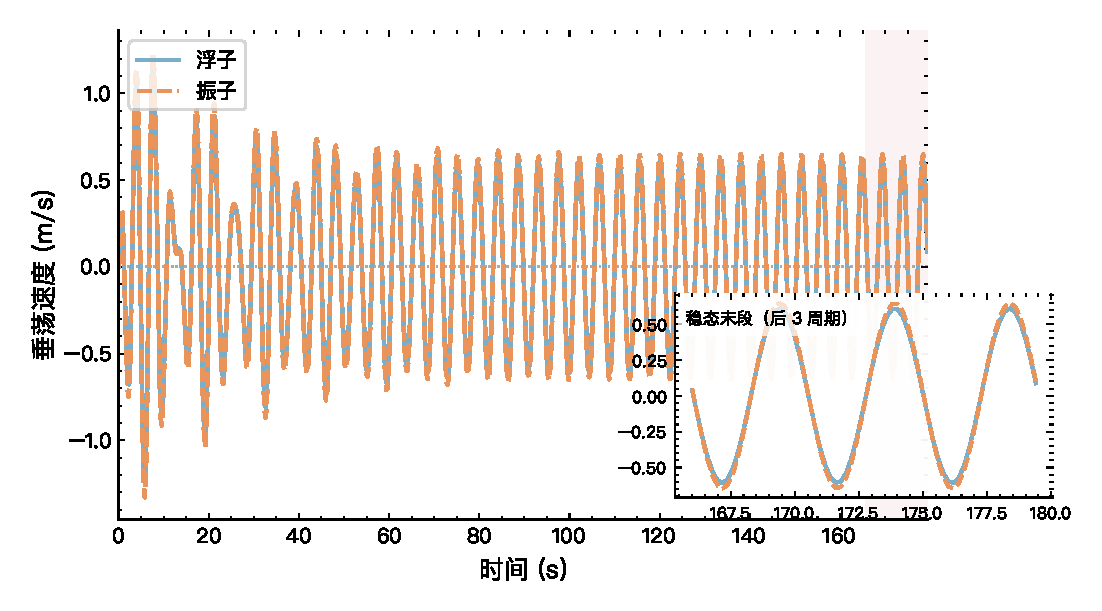
\includegraphics[width=0.85\textwidth]{figures/fig_2_heave_velocity.pdf}
    \caption{浮子与振子垂荡速度时程（前 40 个波浪周期，线性阻尼）}
    \label{fig:heave_velocity}
\end{figure}

% ---- 图 3：相对位移与相对速度时程 ----
\begin{figure}[H]
    \centering
    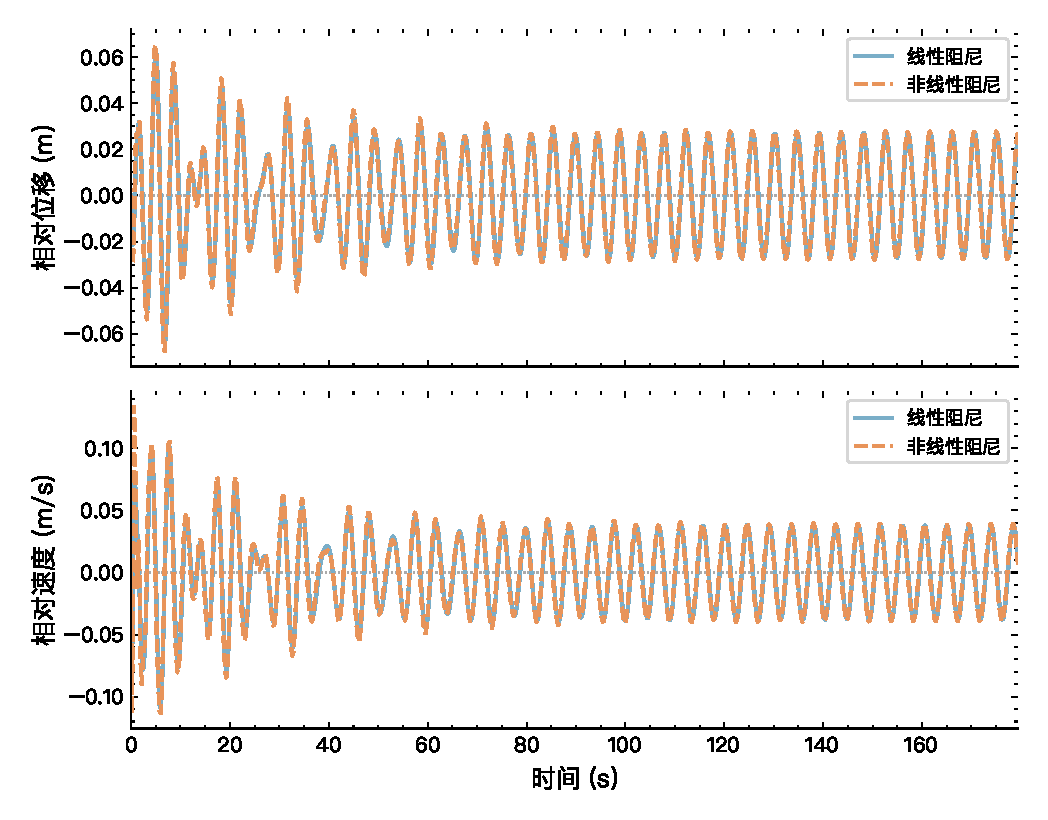
\includegraphics[width=0.85\textwidth]{figures/fig_3_relative_motion.pdf}
    \caption{浮子与振子相对位移及相对速度时程（线性与非线性阻尼对比）}
    \label{fig:relative_motion}
\end{figure}

% ---- 图 4：PTO 瞬时功率曲线 ----
\begin{figure}[H]
    \centering
    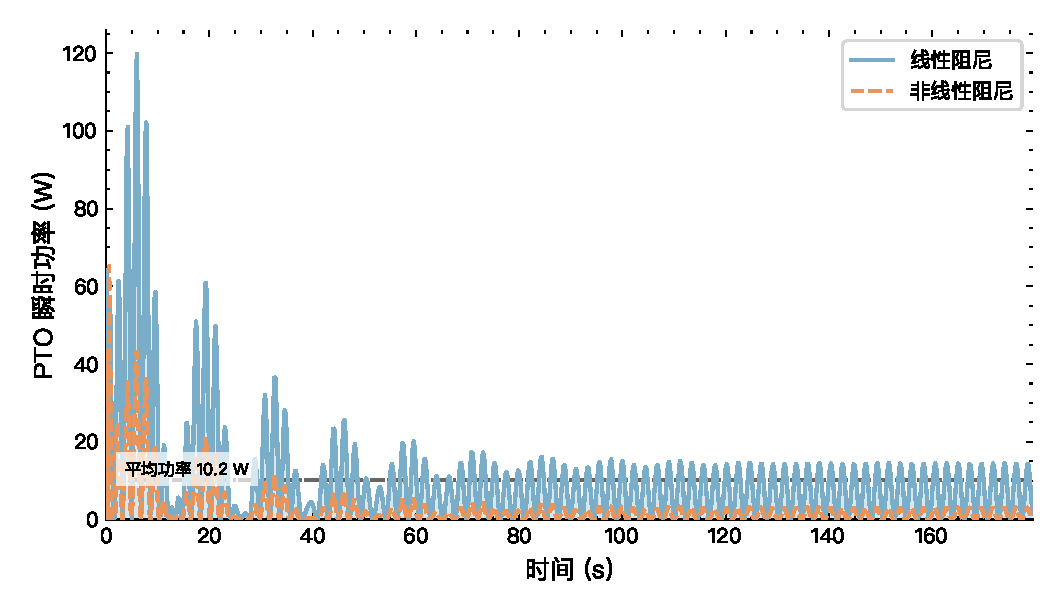
\includegraphics[width=0.85\textwidth]{figures/fig_4_pto_power.pdf}
    \caption{PTO 瞬时输出功率曲线（线性与非线性阻尼对比）}
    \label{fig:pto_power}
\end{figure}

% ---- 表 1：优化结果汇总 ----
% 各子问题能量输出优化结果汇总
\begin{table}[H]
\centering
\caption{各子问题能量输出优化结果汇总}
\label{tab:opt_summary}
\begin{tabular}{lcc}
\toprule
子问题 & 最优阻尼 & 最大平均输出功率 (W) \\
\midrule
问题2（线性） & $C^*=3.72\times10^4$ N·s/m & 229.334 \\
问题2（非线性） & $\alpha^*=1.0\times10^5$, $P^*=0.417$ & 229.980 \\
问题4（直线） & $C_z^*=5.92\times10^4$ N·s/m & 318.336 \\
问题4（旋转） & $C_\theta^*=1.0\times10^5$ N·m·s & 0.011 \\
\midrule
问题4 合计 & — & 318.347 \\
\bottomrule
\end{tabular}
\end{table}


% ---- 表 2：问题1 指定时刻快照 ----
% 问题1 指定时刻浮子/振子位移与速度快照（线性阻尼）
\begin{table}[H]
\centering
\caption{问题1 指定时刻浮子与振子位移/速度快照（线性阻尼 $C=10^4$ N·s/m）}
\label{tab:snapshot}
\resizebox{\textwidth}{!}{%
\begin{tabular}{lcccc}
\toprule
时间 $t$ (s) & 浮子位移 (m) & 浮子速度 (m/s) & 振子位移 (m) & 振子速度 (m/s) \\
\midrule
10  & $-0.1907$ & $-0.6410$ & $-0.2117$ & $-0.6940$ \\
20  & $-0.5907$ & $-0.2410$ & $-0.6342$ & $-0.2728$ \\
40  & $0.2854$  & $0.3130$  & $0.2965$  & $0.3329$  \\
60  & $-0.3145$ & $-0.4795$ & $-0.3314$ & $-0.5157$ \\
100 & $-0.0836$ & $-0.6042$ & $-0.0841$ & $-0.6430$ \\
\bottomrule
\end{tabular}}
\end{table}

